\documentclass[11pt]{article}

\usepackage[margin=1in]{geometry}
\usepackage[T1]{fontenc}
\usepackage[utf8]{inputenc}
\usepackage{amsmath}
\usepackage{amssymb}
\usepackage{booktabs}
\usepackage{array}
\usepackage{microtype}
\usepackage{graphicx}
\usepackage[colorlinks=true, linkcolor=blue, urlcolor=blue, citecolor=blue]{hyperref}
\usepackage{xurl}
\urlstyle{same}

\newcommand{\bibentry}[1]{\par\noindent\hangindent=1.5em\hangafter=1 #1\par\vspace{2pt}}
\newcommand{\doilink}[1]{\href{https://doi.org/#1}{\nolinkurl{doi:#1}}}

\title{The Gate Stopped Deciding: Embedding-Cosine Meaning Gates on Institutional Labels and at Deployment Length}
\author{Scott E. Frias\\ Eigenforma \textperiodcentered\ Freemind Labs\\ \texttt{scott@eigenforma.com}}
\date{August 27, 2026}

\begin{document}

\maketitle

\begin{center}
\small Draft v3.0 (2026-08-27), circulated for author review before arXiv submission. Every quantitative claim below regenerates deterministically from frozen artifacts with a single command (\path{scripts/recompute_headline_numbers.py}, 65 of 65 PASS); bar arithmetic derives strictly from \path{results/verification/bar_ledger.json}. Companion study cited as Frias (2026), arXiv:2608.10216.
\end{center}

\begin{abstract}
Many popular agent frameworks gate meaning with a cosine threshold. Deduplication filters, semantic caches, drift guards, and answer graders all decide whether two texts mean the same thing by thresholding cosine similarity. A companion audit of 80 authored pairs showed the gate class measures \emph{wording}, not meaning (Frias, 2026). We evaluate the same gates on institutional verifications and at production chunk defaults.

Across 25 years of IETF errata verifications, shipped thresholds approved 89--98\% of corrections the institution's own verifiers had ruled as meaning changing, and none of nine encoders exceeded stratified AUROC 0.5237 on the verified classes. Audited span by span against a semantic construct, the labels cap observable AUROC at 0.646 (95.2\% Technical precision, a 66.0\% Editorial leak). On the adjudicated primary corpus, every encoder's confidence interval overlapped the token-Jaccard baseline (0.772), and the production configuration scored 0.714, below it.

Titrating 959 crowdsourced reversal and paraphrase pairs through byte-identical host passages (2,184,150 scored pairs), the critical length $L^*(0.75)$ was left-censored below the shortest buildable passage ($L \le 64$) in all ten configurations. By $L = 256$, eight of ten reached a reversal miss rate of exactly 1.000 and a false-block rate of exactly 0.000 at every operating point to 0.85. The gate degenerated into a constant function returning ``same.'' Chunk defaults sit 6.3--8.0 times beyond the last length ($L = 128$) where any configuration held AUROC 0.55.

Of 21 pre-registered bars, 13 failed outright, one failed at its certification clause, one is unresolved, and three passed only for the configurations able to evaluate them. A transfer prediction failed by improving. A refutation blinded to source showed coupling direction does not invert under a uniform rubric, and magnitude varies severalfold across revision processes.
\end{abstract}

\section{What a threshold asserts}

Agent frameworks built on language models increasingly gate meaning with similarity scores. Deployed architectures use these gates for semantic prompt caching, retrieval deduplication, drift guards on tool arguments, and automated answer grading. Each computes text embeddings $\mathbf{e}(x_1), \mathbf{e}(x_2)$ and accepts or rejects semantic equivalence by whether cosine similarity clears a fixed scalar threshold $\tau$:
\[
S(x_1, x_2) = \frac{\mathbf{e}(x_1) \cdot \mathbf{e}(x_2)}{\|\mathbf{e}(x_1)\| \|\mathbf{e}(x_2)\|} \ge \tau
\]

Our companion study (\hyperlink{bib:frias}{Frias, 2026}) surveyed these gates across open agent frameworks and audited them on an authored instrument of 80 pairs. In that survey, a production drift guard fired on 0 of 56 mutations that break meaning, balanced accuracy never exceeded 0.700 in any of the 90 cells crossing configuration, threshold, and task, and surface lexical overlap confounded the measurements. That audit left two questions open: the two strongest of nine configurations \emph{did} separate negation reversals from paraphrases at matched lexical overlap, with AUROC between 0.79 and 0.90, but whether that separation survives outside the instrument was unmeasured. All 80 pairs were authored by the investigators as isolated single sentences, so nothing spoke to authentic labels or realistic length.

When a deployed system sets its threshold at $\tau = 0.85$ and blocks inputs below it, it asserts a monotonicity: lower cosine similarity means a higher probability of semantic mutation. Nothing intrinsic to the embedding model secures that assertion, and it either holds or fails with the joint distribution of wording distance and semantic change in text the system processes. No deployed gate observes that distribution directly. This paper evaluates the assertion in two domains synthetic benchmarks cannot reach: the historical labels of an engineering standards institution across 25 years, and the passage lengths production systems compare.

\section{Related work}

Nine lines of prior work bear on this study. We state what each showed, then what remained unmeasured. Every characterization in this section was checked against its primary source before release.

\subsection{Auditing the vector-matching layer}

\hyperlink{bib:wangmetmap}{Wang et al.\ (2024)} introduced MeTMaP, the nearest prior systematic probe of the vector-matching layer. It is a metamorphic testing framework that builds sentence triplets from eight metamorphic relations derived from six NLP datasets and runs them against 203 vector-matching configurations (29 embedding models $\times$ 7 distance metrics). Matching accuracy fell by more than 78\% on average relative to the original datasets, with the best of all 203 combinations reaching only 41.51\%; the figure describes the audited configurations, not the measurer.

\hyperlink{bib:steck}{Steck et al.\ (2024)} approached the same instrument analytically. For embeddings from regularized linear models (where closed-form solutions are available) they derived that cosine similarity can yield arbitrary and therefore meaningless similarities, non-unique for some models, and implicitly controlled by the regularization for others. They further argued by extension that the combinations of regularization used in deep models have implicit and unintended effects on the resulting cosine similarities. Both studies ask whether the score means what it is taken to mean, but neither investigated the operational behavior of the binary decision \emph{thresholds} deployed on top of those scores.

\subsection{Length, position, and passage dilution}

Three studies measured how length and position degrade embedding geometry. \hyperlink{bib:zhou}{Zhou et al.\ (2025)} showed that the embeddings of longer texts cluster together (a phenomenon they named Length Collapse), producing a distributional inconsistency between short- and long-text embeddings. They attributed the mechanism to self-attention acting as a low-pass filter whose strength intensifies with length, and proposed TempScale, which applies a temperature coefficient to the attention logits before the softmax. \hyperlink{bib:lyu}{Lyu et al.\ (2026)} identified document-side early compression as a failure mode of single-vector dense retrieval, then introduced the Evidence Dilution Index to measure how far a document-level representation falls below the strongest chunk-level evidence in the same gold document, and ultimately offered DICE, a training-free remedy that encodes chunks independently before aggregating them. \hyperlink{bib:lee}{Lee et al.\ (2024)} documented systematic positional bias in text embedding models irrespective of their positional encoding mechanism, finding that inserting irrelevant text or removing content at the beginning of a document reduces cosine similarity to the original embedding by up to 12.3\% more than the same modification at the end.

These studies establish that context length degrades the geometry, and evaluate the damage on aggregate retrieval rankings (nDCG on MTEB or LongEmbed) or on global dispersion rather than on whether a discrete semantic \emph{decision} survives passage context.

\subsection{Negation and semantic representation failure}

The vulnerability of language models to negation has been established across multiple NLP benchmarks. \hyperlink{bib:hossain}{Hossain et al.\ (2020)} demonstrated two properties of the major Natural Language Inference (NLI) benchmarks, namely, that negation is underrepresented in them, and that the negations that do appear can often be ignored without changing the correct inference. They then constructed pairs of premise and hypothesis in which negation was critical, and transformers at the state of the art struggled on them. \hyperlink{bib:ravichander}{Ravichander et al.\ (2022)} introduced CondaQA, collecting for each negated statement in a Wikipedia passage three edits from crowdworkers: a paraphrase of the negation, a change to its scope that retains the negation cue, and an affirmative edit that undoes it. The dataset holds 14,182 questions with answers over 1,289 passages. \hyperlink{bib:weller}{Weller et al.\ (2024)} derived contrastive document pairs from CondaQA in which only negation differs, then paired them with newly crowdsourced queries to form NevIR, and found every bi-encoder they tested at or below the 25\% random baseline. \hyperlink{bib:vandenelsen}{Van den Elsen et al.\ (2025)} reproduced that result, then extended the analysis to listwise LLM re-rankers, and showed via ExcluIR that fine-tuning gains on one negation benchmark do not transfer to the other.

Several specialized modeling strategies answer this. \hyperlink{bib:anschutz}{Ansch\"utz et al.\ (2023)} found that learned evaluation metrics built on language models, BLEURT, BERTScore, and sentence-transformer cosine similarities among them, barely change their scores when a sentence is negated, and answered with the CANNOT dataset, NegBLEURT, and the NegMPNet encoder. \hyperlink{bib:truong}{Truong et al.\ (2025)} contrastively fine-tuned MPNet on negation and hedging triples distilled from a language model, producing HedgeMPNet, and showed that the same recipe transfers to encoders built on large language models. In clinical NLP, \hyperlink{bib:chapman}{Chapman et al.\ (2001)} published NegEx, a simple algorithm of regular expressions that identifies negated findings in medical discharge summaries, long the standard baseline for negation detection in that domain. That literature answers negation with targeted modeling; this study measures what general-purpose embedding models do with negation once it sits inside a realistic host passage.

\subsection{Empirical validity ladders and evaluation benchmarks}

The validity ladder of \S6 rests on four benchmark corpora with distinct construction methods. For SNLI and MultiNLI, \hyperlink{bib:bowman}{Bowman et al.\ (2015)} and \hyperlink{bib:williams}{Williams et al.\ (2018)} had crowdworkers author hypotheses against existing premises, while Quora released Question Pairs (QQP), a dataset of duplicate questions distributed in GLUE (\hyperlink{bib:wangglue}{Wang et al., 2018}). All three carry elicited pairs, or pairs derived from telemetry, whose target classes correlate naturally with surface lexical overlap.

In contrast, \hyperlink{bib:zhang}{Zhang et al.\ (2019)} constructed PAWS (Paraphrase Adversaries from Word Scrambling), generating 108,463 pairs via controlled word swapping and back-translation, labeled by human raters, so that paraphrase and non-paraphrase pairs alike show high lexical overlap. An encoder can score as discriminative on an elicited benchmark by exploiting surface correlations alone, and the ladder's lower tiers exist to control for that.

\subsection{Deployed threshold calibration and semantic caching}

Static thresholding in production LLM caching systems has recently come under scrutiny. \hyperlink{bib:schroeder}{Schroeder et al.\ (2026)} argued in vCache that a static similarity threshold gives no formal correctness guarantee across prompt distributions, yields unexpected error rates, and produces suboptimal cache hit rates. They replaced it with a threshold learned online per cached prompt under user-defined error rate guarantees. \hyperlink{bib:baral}{Baral et al.\ (2026)} framed model selection for semantic caching as a calibration problem rather than a ranking one, introducing P-CHR AUC and the Calibration Retention Rate to measure it. Both establish that static thresholds do not generalize across prompts; this study evaluates the static gates as shipped, on institutional labels and across length.

\subsection{Institutional labels and specification corpora}

Engineering standards bodies keep rich corpora of authentic revisions. \hyperlink{bib:mcquistin}{McQuistin et al.\ (2023)} performed the first study of the RFC errata process, characterizing the 6,759 errata reports filed between January 2001 and December 2022 by metadata and process outcome and evaluating three strategies for reducing errata. They never applied classifiers to the content of the reports. They also recorded the observation this paper's label noise arm was built around, as erratum 5595 flags a missing ``not'' in a specification. They noted it was arguably editorial, though filed as technical, given that it fundamentally alters the meaning of the text.

Elsewhere, \hyperlink{bib:chen}{Chen et al.\ (2022)} applied fine-tuned BERT embeddings and positive-unlabeled learning in their CREEK pipeline to 3GPP change requests (using the institutional correction category only as a pre-filter, never a feature or label) and recovered 1,270 security-relevant changes from a corpus of 414,488. \hyperlink{bib:nikbakht}{Nikbakht et al.\ (2024)} released TSpec-LLM, an open dataset covering 3GPP documents from Release 8 through Release 19, with a set of technical questions and a retrieval baseline over it. \hyperlink{bib:shen}{Shen et al.\ (2025)} released RFC2PSM, a dataset of 1,580 pages of cleaned RFC specifications across 14 protocols, and PSMBench, the benchmark built over it for protocol state machine extraction. Standards text is an established NLP domain, and this study evaluates verified RFC errata and revision documents as an institutional benchmark for semantic change detection.

\subsection{Construct validity and measurement theory}

\hyperlink{bib:jacobs}{Jacobs and Wallach (2021)} formalized measurement theory for computational systems, locating validity failure in the step where an unobservable construct is operationalized through a proxy measurement model. \hyperlink{bib:li}{Li et al.\ (2026)} defined the \emph{Proxy Presumption} in social NLP as the unwarranted assumption that unsupervised geometric properties like cosine similarity directly measure complex target constructs, while vector distances remain entangled with confounding attributes of style, syntax, and length. This study treats cosine thresholding as that kind of proxy, and tests its construct validity empirically.

\hyperlink{bib:pearson}{Pearson et al.\ (1899)} anticipated reversals of association across aggregated subgroups, \hyperlink{bib:simpson}{Simpson (1951)} set them out in contingency tables, and \hyperlink{bib:blyth}{Blyth (1972)} gave them the name Simpson's Paradox. \hyperlink{bib:yule}{Yule (1903)} analyzed the adjacent hazard, namely, association \emph{created} by amalgamating heterogeneous records, rather than reversed. A similarity benchmark that fails to control subpopulation text distributions can produce the same misleading or inverted conclusions.

\subsection{Representation levels and anisotropy in representation space}

The anisotropy literature reports that transformer representations cluster within a narrow cone. \hyperlink{bib:ethayarajh}{Ethayarajh (2019)} demonstrated that contextualized \emph{token} representations across BERT, ELMo, and GPT-2 occupy narrow cones in upper layers. \hyperlink{bib:gao}{Gao et al.\ (2019)} analyzed representation degeneration in the tied output embedding matrices of generation models and proposed a regularization that encourages isotropic dispersion.

Both findings describe hidden states at the token level and output vocabulary projections. In \S7 we show that pooled manifolds of sentence embeddings do not universally inherit the narrow cone, and a threshold floor derived from token anisotropy fails to carry over.

\subsection{What remained unmeasured}

The literature establishes that cosine similarity can be geometrically distorted, that context length degrades representation fidelity, that negation breaks bi-encoders, that static thresholds fail across prompt distributions, and that unsupervised vector proxies require construct validation. What none of it measured is whether embedding-cosine thresholding survives as a semantic gate on authentic institutional labels and at realistic passage lengths. That measurement is this paper.

\section{Method: pre-registration as the unit of work}

All four experiments were pre-registered under cryptographic freeze tags, and 21 numbered bars with explicit numeric thresholds were committed before any encoder scored any pair, so no hypothesis in this paper was constructed after its evidence. Every corpus was fetched once, hashed into a manifest, and never altered afterward. Every quantitative figure in this manuscript regenerates deterministically from the frozen artifacts via \path{scripts/recompute_headline_numbers.py}. Analysis pipelines went under version control before observation. When an algorithmic defect surfaced after collection, as the caliper permutation indexing defect in \S6 did, the affected verdict was voided, documented, and re-evaluated under a dated amendment rather than silently corrected.

Two independent annotator seats evaluated every audited sample. Both seats were language model instances: one a firewalled context from a commercial frontier model, the other a locally hosted open-weight model from a distinct model family. Machine labels remained sealed until all verdicts were recorded, and remaining disagreements were resolved by manual adjudication. Human replication has not occurred. That boundary covers every metric derived from labels in this paper and is restated wherever one is reported.

\section{The institutional audit}

\textbf{Corpus.} The RFC Editor errata database, frozen on 2026-08-05 and re-verified as byte-identical against the live repository three days later, contains 7,991 entries. From these, 1,425 Technical and 1,402 Editorial prose pairs survive after excluding corrections that are primarily code. Within this taxonomy, \emph{Technical} denotes an error in the normative technical content of the standard, whereas \emph{Editorial} denotes spelling, grammar, or formatting adjustments that preserve technical meaning. Thousands of independent reporters and rotating document verifiers assigned these labels across 25 years, with no knowledge of this study.

\textbf{Lexical confounder balance.} Token-Jaccard medians were 0.889 for Technical corrections and 0.913 for Editorial corrections, a Cliff's $\delta = -0.1005$. This is negligible by standard convention, and oriented in the benign direction, as Technical corrections reword slightly more. The overlap balance that synthetic instruments must build by hand arises here from the ordinary editing process.

\textbf{Gate performance on archival labels.} At the standard operating point of $\tau = 0.80$, the gates approved between 89\% and 98\% of Verified-Technical corrections; hypothesis $H_1$'s pre-registered approval bar of at least 90\% was missed narrowly on two configurations (89.3\% and 89.7\%). Marginal AUROC ranged from 0.5525 to 0.5693. The certification clause failed on three configurations, with marginal movements between 0.046 and 0.050, and triggered the pre-registered fallback to stratified estimation. Under that fallback, no configuration exceeded an AUROC of \textbf{0.5237}. Fitted optimal thresholds ranged from $\tau = 0.989$ to 0.997 with in-sample balanced accuracy of only 0.546 to 0.558. Even optimized directly on in-domain data, a single threshold separates verified institutional corrections at negligible capacity.

\textbf{Construct label audit and noise ceiling.} Two blinded annotator seats evaluated 300 stratified pairs against a span-level semantic construct, without access to the official IETF classification, and agreed at Cohen's $\kappa = 0.6813$. All 34 disagreements were adjudicated by hand. Technical label precision was 95.2\%, perfect on the two categories prior audits emphasized (47 of 47 requirement keyword modifications and 49 of 49 numerical quantity modifications). However, 66.0\% of Editorial corrections were adjudicated as changing meaning at the span level, because the institutional label reflects standardization at the document level rather than the semantics of the local span. This label attenuation caps the maximum observable AUROC on these institutional labels at \textbf{0.646}, and every decision metric in this section reads against that ceiling.

\textbf{Primary corpus promotion.} Because construct disagreement on the Editorial class substantially exceeded the pre-registered 15\% threshold, the adjudicated subsample was promoted to the primary evaluation corpus. Under span construct labels, the nine encoders scored AUROC between 0.714 and 0.804, while simple token-Jaccard lexical overlap scored 0.772. Cluster bootstrap 95\% confidence intervals for all nine encoders overlapped the Jaccard baseline. Reweighted to the full Verified-prose frame, encoder AUROC ranged from 0.669 to 0.761 against a reweighted Jaccard baseline of 0.730. On both label axes embedding similarity failed to beat lexical overlap, and the deployed production configuration finished below a baseline that counts words (Figure~\ref{fig:baseline}).

\begin{figure}[t]
\centering

\includegraphics[width=0.92\linewidth]{figures/fig1_word_counting_baseline.pdf}
\caption{Encoder AUROC against the span-level construct labels on the adjudicated primary corpus, with the token-Jaccard word-counting baseline and the deployed production configuration marked (\S4).}
\label{fig:baseline}
\end{figure}

\textbf{Semantic classes and a class inversion.} A tiered cascade classified all 1,425 Technical pairs into five semantic classes, with 556 ambiguous pairs arbitrated blindly by a frontier model. Across nine configurations, numerical quantity modifications showed median cosine similarities between 0.991 and 0.999, the \emph{least} detectable class in 9 of 9 configurations. Polarity and negation corrections produced medians between 0.980 and 0.994, while modal keyword modifications ranged 0.928 to 0.985, the most detectable in 9 of 9. This inverts the class ordering of the synthetic instrument, where modal changes were least detectable, so per-class detectability follows corpus composition rather than encoder inductive bias. Across the 36 corrections the IETF verified as authentic technical errors and the cascade filed as polarity, median cosine similarity ran 0.980 to 0.994, and the deployed production path scored them at 0.993.

\textbf{Transfer to working-group revisions.} We fitted repair models on errata pairs, froze their parameters, and evaluated transfer on an aligned corpus of 13,780 sentence pairs mined from 1,542 revision documents that carry an RFC to its bis successor, 2,019 transitions in requirement strength among them. Hypothesis $H_4$ pre-registered a drop of at least 0.10 AUROC. Every fitted model improved instead: fixed thresholds gained 0.03 to 0.06 balanced accuracy, and the logistic gate gained 0.14 to 0.17, reaching AUROC between 0.71 and 0.74 across all nine configurations. Uniform improvement across nine distinct architectures reflects lexical separation shared at the corpus level rather than learned semantics. The pre-registered bar failed by improving; an engineer validating across these corpora would have observed a gain and deployed the gate.

\section{At deployment length}

\textbf{Instrument design.} We sampled 959 anchor sets from CondaQA (\hyperlink{bib:ravichander}{Ravichander et al., 2022}), crowdsourced originally for negation comprehension. Each anchor set holds an original sentence, a paraphrase that preserves its meaning, and an affirmative edit that inverts the negation; a set was retained only where both edits recover as strict replacements of one sentence in the same slot of the original. Each payload was spliced into authentic host documents, with Wikipedia as the primary domain and PubMed Central and the RFC corpus held out. Both members of every evaluated pair share byte-identical host context at identical relative positions, so passage length is the only variable. We titrated nominal passage lengths from $L = 64$ to $L = 4{,}096$ whitespace tokens at three insertion positions, and scored 2,184,150 pairs over ten configurations. Eight configurations matched the pinned reference path within absolute tolerances of $10^{-7}$ to $10^{-6}$; two ran under a declared amendment covering fresh numerics, with maximum cosine deviations of $3.63 \times 10^{-4}$ and $4.47 \times 10^{-4}$.

\textbf{Empirical results.} Table~\ref{tab:titration} reports decision AUROC, flip against faithful, pooled across positions on Wikipedia host passages, and Figure~\ref{fig:dilution} traces the decay:

\begin{table}[t]
\centering
\footnotesize
\setlength{\tabcolsep}{4pt}
\begin{tabular}{lcccccc}
\toprule
configuration & 64 & 128 & 256 & 512 & 1024 & 4096 \\
\midrule
mxbai-embed-large-v1 & 0.605 & 0.550 & 0.532 & 0.512$^\dagger$ & 0.500$^\dagger$ & 0.501$^\dagger$ \\
e5-base-v2 [query:] & 0.602 & 0.550 & 0.524 & 0.505$^\dagger$ & 0.498$^\dagger$ & 0.501$^\dagger$ \\
bge-base-en-v1.5 & 0.551 & 0.511 & 0.502 & 0.504$^\dagger$ & 0.498$^\dagger$ & 0.501$^\dagger$ \\
nomic clustering, long-context 8192 & 0.550 & 0.543 & 0.534 & 0.527 & 0.520 & 0.509 \\
nomic clustering (same checkpoint) & 0.550 & 0.543 & 0.534 & 0.527 & 0.520 & 0.509 \\
e5-base-v2 [no prefix] & 0.542 & 0.514 & 0.505 & 0.499$^\dagger$ & 0.497$^\dagger$ & 0.501$^\dagger$ \\
all-mpnet-base-v2 & 0.538 & 0.527 & 0.526 & 0.508$^\dagger$ & 0.503$^\dagger$ & 0.502$^\dagger$ \\
gte-base & 0.523 & 0.505 & 0.500 & 0.500$^\dagger$ & 0.498$^\dagger$ & 0.502$^\dagger$ \\
nomic-MRL-256, production & 0.517 & 0.520 & 0.522 & 0.519 & 0.515 & 0.508 \\
all-MiniLM-L6-v2 & 0.490 & 0.497 & 0.494$^\dagger$ & 0.497$^\dagger$ & 0.500$^\dagger$ & 0.500$^\dagger$ \\
\bottomrule
\end{tabular}
\caption{Decision AUROC, flip against faithful, by nominal passage length (whitespace tokens), positions pooled, Wikipedia hosts. The dagger marks cells where the spliced passage exceeds the encoder's operative context window (\S5).}
\label{tab:titration}
\end{table}

All ten configurations appear, and the two nomic clustering rows share one checkpoint, so their values are identical.

\begin{figure}[t]
\centering

\includegraphics[width=0.92\linewidth]{figures/fig2_dilution_decay.pdf}
\caption{Decision AUROC, flip against faithful, against passage length, positions pooled, Wikipedia hosts. Dashed segments and hollow markers denote cells where the passage exceeds the encoder's operative window (\S5, Table~\ref{tab:titration}).}
\label{fig:dilution}
\end{figure}

\textbf{Context window truncation ($\dagger$).} The dagger marks cells where the spliced passage exceeded the encoder's maximum context window. In these cells the metric is not a measurement at the nominal column length; the encoder truncated the passage and rescored a fixed window. Seven of the ten configurations truncate from $L \ge 512$, and at $L = 1024$ and $L = 4096$ every evaluated pair is truncated, so scores at those lengths report window ceilings rather than continuous length decay. Model \texttt{all-MiniLM-L6-v2} truncates from $L = 256$. Only the three nomic configurations, with a context window of 8,192 tokens, stay within window across the full sweep.

\textbf{Critical discrimination length.} The critical discrimination length $L^*(0.75)$, the maximum length that sustains an AUROC $\ge 0.75$, was left-censored at or below $L \le 64$ tokens for all ten configurations: no evaluated encoder discriminated usably at the shortest passage the instrument could build. Relaxed to $L^*(0.55)$, five configurations stayed censored below $L \le 64$, and the rest crossed at 65.8, 103.8 (both nomic variants), 127.3, and 129.6 nominal tokens.

\textbf{A pre-registered bridge to the ranking setting.} The pre-registration committed to a descriptive bridge to the ranking results of \hyperlink{bib:weller}{Weller et al.\ (2024)}: a pairwise accuracy in NevIR's style on the shortest cell, the fraction of (anchor, position) cells in which the reversal scores a lower cosine than the paraphrase, ties counted 0.5. On the $L = 64$ Wikipedia cell, pairwise accuracy spans 0.494 to 0.680 across the ten configurations: highest for \texttt{mxbai} at 0.680, the deployed production path at 0.542, and \texttt{all-MiniLM-L6-v2} at 0.494, below the 0.5 chance level of the pairwise metric. The two settings are not directly comparable, as NevIR's random baseline for its own ranking metric is 25\%, and the bridge is reported as a descriptive anchor only.

These measurements resolve the open question of the synthetic audit. On single sentences, \texttt{mxbai} separated reversal from paraphrase at an AUROC of 0.895; embedded in a short paragraph of $L = 64$ tokens, that separation fell to \textbf{0.605}, and by $L = 512$ it read 0.512. Discrimination that exists in an isolated sentence does not survive its surrounding context.

\textbf{Gate degeneracy in deployed systems.} In operational terms, the critical length at which the reversal miss rate reaches 0.99 across all operating points $\tau \le 0.85$ was $L = 64$ for every configuration. By $L = 256$ tokens, eight of the ten configurations reached a reversal miss rate of exactly 1.000 with a faithful false-block rate of exactly 0.000 across all thresholds $\tau \le 0.85$; a ninth reached 0.9985, and the tenth truncated before 256 tokens. At this length the gate had stopped discriminating inputs, and had degenerated into a constant function returning ``same.''

\textbf{Comparison with production chunk sizes.} Default chunk sizes in standard agent frameworks run 1,024 tokens in LlamaIndex, 1,000 tokens in Microsoft Kernel Memory, and 4,000 characters ($\approx 800$ whitespace tokens) in LangChain's recursive text splitter; each default was read from the shipped package or its documentation before the length grid froze, with provenance recorded in \path{docs/e2_pretag_provenance.md}. The longest passage at which any configuration held an AUROC $\ge 0.55$ was $L = 128$. Production deployments therefore run \textbf{6.3 to 8.0 times} beyond the point where any evaluated gate keeps marginal discrimination ($800/128 = 6.25\times \approx 6.3\times$; $1000/128 = 7.8125\times \approx 7.8\times$; $1024/128 = 8.0\times$).

\textbf{Does escalating to a language model judge escape the decay?} The natural answer to a failing embedding gate is to escalate the decision to a language model. We tested that answer at matched conditions on the same frozen corpus: 1,440 judgments from two instruction-tuned models of different families (Qwen3.8-27B and Mistral-Small-24B), across both the Wikipedia and RFC host registers and all eight lengths, at temperature zero, with every reply parsed and none discarded. A judge emits a binary verdict rather than a score, so it occupies a single operating point; the reported quantity is the area of that one-point ROC, $(\mathrm{TPR} + \mathrm{TNR})/2$, comparable to the encoder curves in level and in shape but not sweepable to another threshold without changing the prompt.

The judge ran well above every encoder and decayed the same way (Figure~\ref{fig:llmjudge}). Its discrimination was 0.817 (95\% CI $[0.755, 0.878]$) at $L = 64$ and 0.567 ($[0.491, 0.642]$) at $L = 4096$, where the interval includes chance. Its interval sits strictly above the 0.75 line for usable discrimination only at $L = 64$ and $L = 96$, and no encoder configuration reaches 0.75 at any length. Escalation therefore moves the ceiling on usable discrimination from nowhere to roughly $L \approx 96$ tokens, and production chunk defaults of 800 to 1,024 tokens remain some eight to ten times beyond even the escalated instrument. The decay belongs to the length regime rather than to thresholded cosine, and raising the instrument raises the level of the curve without changing its shape.

Three limits bound this arm. It used one prompt at one operating point, so its absolute level is a property of that prompt, and a better prompt may sit higher at every length. Its controls are CondaQA paraphrase edits of sentences that carry negation (deliberately the hardest available negatives), so the false-block component is an upper bound. And movement between cells is smaller than the confidence intervals, so the curve reads as a trend between its endpoints rather than as eight independent measurements; we fitted no decay exponent to it.

\begin{figure}[t]
\centering

\includegraphics[width=0.92\linewidth]{figures/fig5_llm_judge_dilution.pdf}
\caption{Flip against faithful discrimination against passage length for a language model judge panel and for two encoder configurations, on the same frozen corpus (SPLICE arm, Wikipedia and RFC hosts, positions pooled). The judge series is the area of a single-point ROC, $(\mathrm{TPR}+\mathrm{TNR})/2$, over 120 mutation and 60 control judgments per length; the shaded band is its 95\% confidence interval. Encoder series are swept AUROC from Table~\ref{tab:titration}; hollow markers and dashed segments denote cells outside the encoder's operative window. The judge sits well above every encoder and falls toward chance across the same range.}
\label{fig:llmjudge}
\end{figure}

\textbf{Pre-registered bar outcomes and structural limits.} Hypothesis $H_{3a}$ predicted a position effect of $\Delta \text{AUROC} \ge 0.05$ and failed in all configurations (0 of 10), with empirical differences spanning $-0.0140$ to $+0.0150$. Six of ten confidence intervals excluded zero, so a minor position effect exists, inconsistent in sign and an order of magnitude below the registered threshold. Hypothesis $H_6$ predicted that power law curves fitted on Wikipedia would capture held-out PMC and RFC cells inside their 90\% prediction intervals; only 69 of 101 evaluable cells fell inside, failing the bar. Seven configurations also have no within-window evaluations at $L \ge 512$, and \texttt{all-MiniLM-L6-v2} none at $L \ge 256$, under their operative window constraints. For these models, dilution at production chunk lengths is moot because \textbf{they truncate before they dilute}, restricting the power law fit to spline approximations and leaving hypothesis $H_1$'s $\alpha$ parameter band unresolved.

\section{Which corpora taught the field that cosine works}

We evaluated nine configurations across SNLI (\hyperlink{bib:bowman}{Bowman et al., 2015}), MultiNLI (\hyperlink{bib:williams}{Williams et al., 2018}), QQP (\hyperlink{bib:wangglue}{Wang et al., 2018}), and PAWS-Wiki, the \texttt{labeled\_final} subset of PAWS (\hyperlink{bib:zhang}{Zhang et al., 2019}), and we positioned the IETF errata corpus as the bottom tier of an empirical validity ladder:

\begin{center}
\small
\begin{tabular}{llcc}
\toprule
tier & corpus & naive AUROC & Jaccard-caliper \\
\midrule
elicited, aligned coupling & SNLI, MNLI, QQP & 0.64 to 0.92 & 0.59 to 0.91 \\
adversarial minimal pairs & PAWS-Wiki & 0.61 to 0.68 & 0.60 to 0.68 \\
natural institutional minimal pairs & IETF errata & 0.55 to 0.57 & 0.50 to 0.52 \\
\bottomrule
\end{tabular}
\end{center}

Every evaluated configuration cleared an AUROC of 0.80 on QQP, spanning 0.85 to 0.90. Embedding-cosine gates perform well where lexical overlap aligns with the target classes, and that regime characterizes the corpora that historically validated cosine matching. We also evaluated, and disproved, the hypothesis that simple overlap matching rectifies elicited benchmarks. Controlling token overlap by caliper matching removed only 0.06 to 0.10 AUROC on QQP and 0.02 to 0.06 on SNLI and MNLI. Elicited pairs differ in stylistic and lexical regularities beyond raw overlap, and embeddings capture those readily, so benchmark validity requires construction from minimal pairs rather than overlap balancing after the fact. PAWS's caliper invariance (maximum shift $\le 0.003$) serves as the empirical positive control for this estimator.

\section{A bound we pre-registered and missed}

In this analysis, a \emph{register} denotes one of three frozen text sets evaluated across all encoders: the errata prose subset ($g_2$), the CondaQA titration passages, and the synthetic brand sentences. If all embeddings within a register lie within an angular radius $\theta$ of the register's mean vector $\boldsymbol{\mu}$, then all pairwise cosine similarities are bounded below by $\cos(2\theta)$:
\[
\mathbf{e}_i \cdot \boldsymbol{\mu} \ge \cos \theta \implies \cos(\mathbf{e}_i, \mathbf{e}_j) \ge \cos(2\theta)
\]
Any operating threshold set below $\cos(2\theta)$ would be geometrically incapable of triggering.

We pre-registered that this geometric floor would constrain low production thresholds, on literature reporting that sentence embeddings cluster in narrow cones. The hypothesis failed. Only \texttt{gte-base} satisfied the $\tau = 0.40$ threshold (1 of 9), none cleared $\tau = 0.60$, and \texttt{bge} produced an empirical minimum similarity of $-0.60$ on CondaQA passages. For \texttt{MiniLM} and \texttt{mpnet}, embeddings extended past orthogonality to the mean vector, reaching maximum angles of $\theta = 106.321^\circ$. For these models the embedding space forms no narrow cone, and the theoretical bound does not apply. The geometric measurement reproduced across distinct GPU architectures within $0.000^\circ$.

The anisotropy literature motivating the pre-registration (\hyperlink{bib:ethayarajh}{Ethayarajh, 2019}; \hyperlink{bib:gao}{Gao et al., 2019}) measured contextualized token representations and tied output embeddings rather than pooled manifolds of sentence embeddings. The hypothesized floor rested on an invalid generalization across representation levels.

\section{Testing cross-source coupling: an empirical refutation}

Prior exploratory analysis suggested that the relationship between lexical overlap and semantic change might reverse direction across text domains. That conjecture rested on comparisons across heterogeneous benchmark rows whose labels came from distinct annotation procedures, so the apparent inversion could have been a labeling difference rather than a property of the text.

We ran a refutation experiment blinded to source, under a single span construct rubric. Two annotator seats agreed at Cohen's $\kappa = 0.6842$ across 380 stratified pairs drawn from three corpora. \textbf{No source came back inverted} (Figure~\ref{fig:coupling}). Lexical overlap differences between preserving and changing pairs measured $+0.081$ for errata (95\% CI $[0.026, 0.148]$), $+0.331$ for bis revisions (95\% CI $[0.256, 0.396]$), and $+0.196$ for the synthetic authored instrument (95\% CI $[-0.542, 0.627]$).

\begin{figure}[t]
\centering
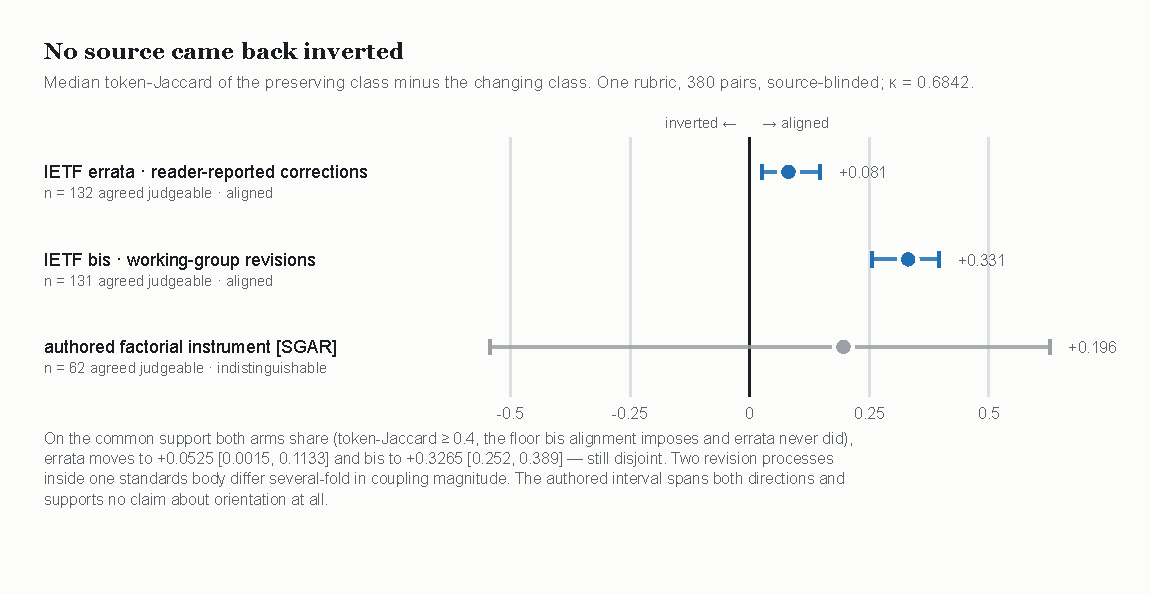
\includegraphics[width=0.88\linewidth]{figures/fig3_no_source_inverted.pdf}
\caption{Lexical overlap differences between meaning-preserving and meaning-changing pairs under the uniform span construct rubric, per source, with bootstrap confidence intervals (\S8).}
\label{fig:coupling}
\end{figure}

The synthetic instrument of \hyperlink{bib:frias}{Frias (2026)} was a balanced $2 \times 2$ factorial design in which lexical overlap was a manipulated factor fixed at ten pairs per cell, so the metrics observed there reflected the design's cell constraints rather than natural properties of an unconstrained authoring process.

The verified finding is that revision processes differ in coupling magnitude rather than orientation. Because bis candidate extraction required a token-Jaccard overlap $\ge 0.40$ while errata extraction applied no overlap filter, we re-evaluated both corpora on their common support ($J \ge 0.40$). The errata difference moved to $+0.0525$ (95\% CI $[0.0015, 0.1133]$) and bis revisions to $+0.3265$ (95\% CI $[0.252, 0.389]$), with confidence intervals that do not overlap. Two revision processes inside one standards organization differ severalfold in coupling magnitude under a uniform semantic construct. We restrict the claim to these observed institutional processes.

\section{The scorecard}

The 21 pre-registered bars are tabulated in the artifact repository and drawn in Figure~\ref{fig:scorecard}. Thirteen bars failed outright, one failed at its certification clause, one remains unresolved, three passed qualified by exclusion or non-evaluability, and three passed cleanly.

\begin{figure}[t]
\centering
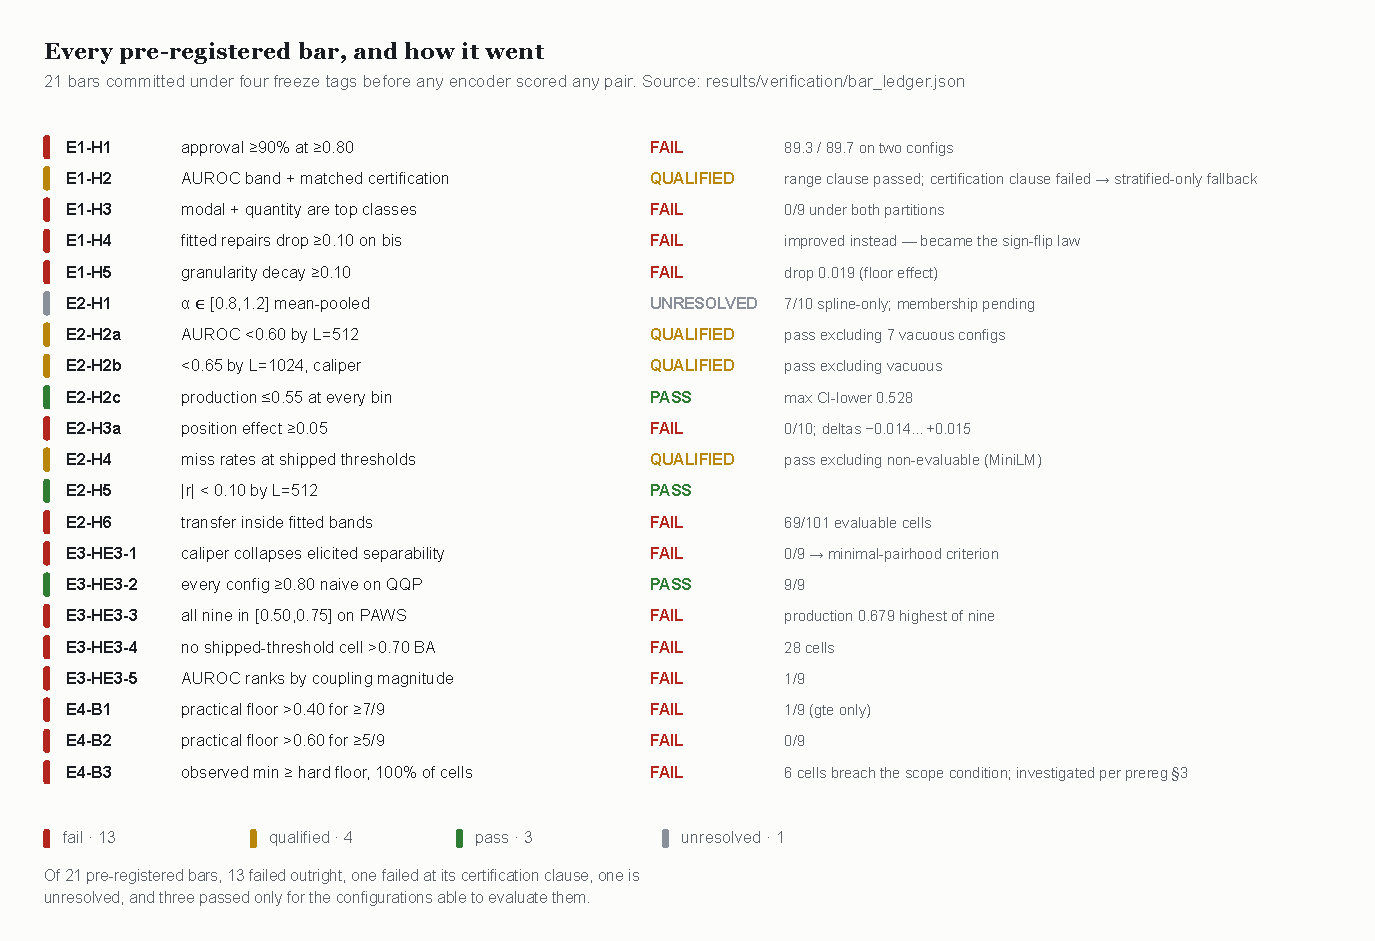
\includegraphics[width=\linewidth]{figures/fig4_scorecard.pdf}
\caption{The 21 pre-registered bars by outcome (\S9). Bar arithmetic derives from the frozen ledger.}
\label{fig:scorecard}
\end{figure}

The aggregate count is the conservative summary of the ledger. Every pre-registered bar asserted one of three conditions: that a failure mode occurs, the magnitude of an effect, or a mechanism. No bar of the first kind failed. All 13 outright failures were wrong predictions of magnitude or mechanism.

Notably, five of the 13 failed because the gates outperformed our registered failure bounds:

\begin{center}
\small
\begin{tabular}{p{1.6cm}p{6.2cm}p{6.2cm}}
\toprule
bar & what we registered & what we measured \\
\midrule
E1-H1 & at least 90\% of Verified-Technical corrections approved at 0.80 & 89.3\% and 89.7\% on two of nine \\
E1-H4 & every repair fitted on errata drops at least 0.10 on bis & every one improved; the logistic gate by 0.14 to 0.17 \\
E3-HE3-1 & the overlap caliper collapses elicited separability & it removed 0.02 to 0.10 of it \\
E3-HE3-3 & the production path scores at most 0.62 on PAWS & 0.679, the highest of the nine \\
E3-HE3-4 & no cell at a shipped threshold exceeds 0.70 balanced accuracy & 28 cells did \\
\bottomrule
\end{tabular}
\end{center}

An evaluation biased toward negative findings does not fail in the direction of higher gate performance on five separate occasions. The remaining eight failures eliminated mechanisms this study proposed: the semantic class hierarchy inverted (0 of 9), the hypothesized position effect was negligible (0 of 10), fitted decay curves failed transfer out of domain (69 of 101 cells), coupling magnitude failed to rank encoder performance (1 of 9), and the geometric cone floor was absent at both registered thresholds (1 of 9 and 0 of 9), breaching its scope condition in six cells.

None of the 13 alters the primary finding. The passing bars and the direct measurements establish that embedding-cosine gates cannot reliably separate variants that change meaning from variants that preserve it; the rejected auxiliary hypotheses simply do not carry that result.

\section{Limitations}

All construct annotations in this study derive from two language model annotator seats with manual adjudication of disagreements; independent human replication has not occurred. The E2 relabeling arm was not executed, so titration AUROC values lack an empirical label noise ceiling (the errata analysis, by contrast, establishes one at 0.646). Seven encoder configurations provide no within-window measurements at $L \ge 512$ tokens under their context window limits. The two nomic clustering configurations share one checkpoint and generate identical curves, so the ten evaluated configurations comprise nine unique models. Host passages and insertion positions were sampled once per anchor set. The bis corpus relies on automated extraction with an estimated positive class precision of 84.8\% and a negative class leak of 37\% (itself a sign that filters on lexical change miss over a third of semantic mutations). Checkpoints specialized for negation (\hyperlink{bib:truong}{Truong et al., 2025}) were not publicly available and appear only in exploratory comparisons. The coupling magnitude findings of \S8 rest on two corpora within a single standards body.

\section{What we release}

We release the complete research artifact: the frozen IETF errata benchmark at three granularities with audited construct labels; the mined RFC requirement change corpus with validation metadata; the full passage titration dataset and its regeneration pipeline with cryptographic checksums; all frozen evaluation scores; the four pre-registration protocols with their amendment logs; the retained vectors of the geometric floor survey; and the verification script that recomputes every headline number deterministically. Synthetic benchmarks have historically lacked empirical verification instruments. This work releases three and confirms that embedding-cosine gates fail to decide meaning.

The class structure of \S4 sets up the successor question. The semantic classes it measured (quantity edits at median cosine 0.991 to 0.999, polarity and negation at 0.980 to 0.994, modal keywords at 0.928 to 0.985) are exact edits local to a span: a number, a negation token, a modal keyword. That family is what an exact span comparison can see \emph{without} a model. Whether a gate built on that asymmetry survives these corpora is a follow-up study in preparation at this lab, to be pre-registered before any encoder scores a pair.

\section*{References}

\noindent{\small The BibTeX source of record is \path{docs/references.bib}; every entry was fetched from a primary source, and the characterization audit trail is \path{docs/reference_verification.md}.}\par\vspace{6pt}

\bibentry{\hypertarget{bib:anschutz}{}Ansch\"utz, M., Miguel Lozano, D., \& Groh, G. (2023). \emph{This is not correct! Negation-aware evaluation of language generation systems.} INLG 2023, 163--175. \doilink{10.18653/v1/2023.inlg-main.12}.}
\bibentry{\hypertarget{bib:baral}{}Baral, A., Ralev, R., Zhechev, I. S., Rajamohan, S., \& Agarwal, J. (2026). \emph{Closing the calibration gap in semantic caching.} arXiv:2606.19719.}
\bibentry{\hypertarget{bib:blyth}{}Blyth, C. R. (1972). \emph{On Simpson's paradox and the sure-thing principle.} Journal of the American Statistical Association, 67(338), 364--366. \doilink{10.1080/01621459.1972.10482387}.}
\bibentry{\hypertarget{bib:bowman}{}Bowman, S. R., Angeli, G., Potts, C., \& Manning, C. D. (2015). \emph{A large annotated corpus for learning natural language inference.} EMNLP 2015, 632--642. \doilink{10.18653/v1/D15-1075}.}
\bibentry{\hypertarget{bib:chapman}{}Chapman, W. W., Bridewell, W., Hanbury, P., Cooper, G. F., \& Buchanan, B. G. (2001). \emph{A simple algorithm for identifying negated findings and diseases in discharge summaries.} Journal of Biomedical Informatics, 34(5), 301--310. \doilink{10.1006/jbin.2001.1029}.}
\bibentry{\hypertarget{bib:chen}{}Chen, Y., Tang, D., Yao, Y., Zha, M., Wang, X., Liu, X., Tang, H., \& Zhao, D. (2022). \emph{Seeing the forest for the trees: Understanding security hazards in the 3GPP ecosystem through intelligent analysis on change requests.} USENIX Security 2022, 17--34.}
\bibentry{\hypertarget{bib:ethayarajh}{}Ethayarajh, K. (2019). \emph{How contextual are contextualized word representations? Comparing the geometry of BERT, ELMo, and GPT-2 embeddings.} EMNLP-IJCNLP 2019, 55--65. \doilink{10.18653/v1/D19-1006}.}
\bibentry{\hypertarget{bib:frias}{}Frias, S. E. (2026). \emph{Similarity gates approve reversals: A validity audit of embedding-cosine thresholds in agent systems.} arXiv:2608.10216. Artifact: github.com/eigenforma/polaritycheck, \doilink{10.5281/zenodo.21796531}.}
\bibentry{\hypertarget{bib:gao}{}Gao, J., He, D., Tan, X., Qin, T., Wang, L., \& Liu, T.-Y. (2019). \emph{Representation degeneration problem in training natural language generation models.} ICLR 2019. \url{https://openreview.net/forum?id=SkEYojRqtm}.}
\bibentry{\hypertarget{bib:hossain}{}Hossain, M. M., Kovatchev, V., Dutta, P., Kao, T., Wei, E., \& Blanco, E. (2020). \emph{An analysis of natural language inference benchmarks through the lens of negation.} EMNLP 2020, 9106--9118. \doilink{10.18653/v1/2020.emnlp-main.732}.}
\bibentry{\hypertarget{bib:jacobs}{}Jacobs, A. Z., \& Wallach, H. (2021). \emph{Measurement and fairness.} FAccT 2021, 375--385. \doilink{10.1145/3442188.3445901}.}
\bibentry{\hypertarget{bib:lee}{}Lee, R. J., Goel, S., \& Ramchandran, K. (2024). \emph{Quantifying positional biases in text embedding models.} arXiv:2412.15241.}
\bibentry{\hypertarget{bib:li}{}Li, B., Yu, T., Koa, K. J. L., \& Huang, K.-W. (2026). \emph{The Proxy Presumption: From semantic embeddings to valid social measures.} ACL 2026. arXiv:2605.07409 (v2).}
\bibentry{\hypertarget{bib:lyu}{}Lyu, S., Wang, Y., Cai, Y., Guo, J., \& Liu, S. (2026). \emph{Lost in a single vector: Improving long-document retrieval with chunk evidence aggregation.} arXiv:2606.18781.}
\bibentry{\hypertarget{bib:mcquistin}{}McQuistin, S., Karan, M., Khare, P., Perkins, C., Purver, M., Healey, P., Castro, I., \& Tyson, G. (2023). \emph{Errare humanum est: What do RFC errata say about Internet standards?} TMA 2023, 1--9. \doilink{10.23919/TMA58422.2023.10198980}.}
\bibentry{\hypertarget{bib:nikbakht}{}Nikbakht, R., Benzaghta, M., \& Geraci, G. (2024). \emph{TSpec-LLM: An open-source dataset for LLM understanding of 3GPP specifications.} IEEE Globecom Workshops 2024, 1--6. \doilink{10.1109/GCWKSHP64532.2024.11101012}.}
\bibentry{\hypertarget{bib:pearson}{}Pearson, K., Lee, A., \& Bramley-Moore, L. (1899). \emph{Mathematical contributions to the theory of evolution. VI. Genetic (reproductive) selection: Inheritance of fertility in man, and of fecundity in thoroughbred racehorses.} Philosophical Transactions of the Royal Society A, 192, 257--330.}
\bibentry{\hypertarget{bib:ravichander}{}Ravichander, A., Gardner, M., \& Marasovi\'c, A. (2022). \emph{CondaQA: A contrastive reading comprehension dataset for reasoning about negation.} EMNLP 2022, 8729--8755. \doilink{10.18653/v1/2022.emnlp-main.598}.}
\bibentry{\hypertarget{bib:schroeder}{}Schroeder, L. G., Desai, A., Cuadron, A., Chu, K., Liu, S., Zhao, M., Krusche, S., Kemper, A., Zaharia, M., \& Gonzalez, J. E. (2026). \emph{vCache: Verified semantic prompt caching.} ICLR 2026. arXiv:2502.03771.}
\bibentry{\hypertarget{bib:shen}{}Shen, Z., Luo, X., Karim, I., \& Bertino, E. (2025). \emph{PSMBench: A benchmark and dataset for evaluating LLMs extraction of protocol state machines from RFC specifications.} NeurIPS 2025 Datasets and Benchmarks Track. \url{https://openreview.net/forum?id=5HGBErIHuV}.}
\bibentry{\hypertarget{bib:simpson}{}Simpson, E. H. (1951). \emph{The interpretation of interaction in contingency tables.} Journal of the Royal Statistical Society: Series B, 13(2), 238--241. \doilink{10.1111/j.2517-6161.1951.tb00088.x}.}
\bibentry{\hypertarget{bib:steck}{}Steck, H., Ekanadham, C., \& Kallus, N. (2024). \emph{Is cosine-similarity of embeddings really about similarity?} WWW '24 Companion, 887--890. \doilink{10.1145/3589335.3651526}. arXiv:2403.05440.}
\bibentry{\hypertarget{bib:truong}{}Truong, T. H., Verspoor, K., Cohn, T., \& Baldwin, T. (2025). \emph{Learning robust negation text representations.} arXiv:2507.12782.}
\bibentry{\hypertarget{bib:vandenelsen}{}van den Elsen, C., Barkhof, F., Nijdam, T., Lupart, S., \& Aliannejadi, M. (2025). \emph{Reproducing NevIR: Negation in neural information retrieval.} SIGIR 2025 Reproducibility Track, 3346--3356. \doilink{10.1145/3726302.3730294}. arXiv:2502.13506.}
\bibentry{\hypertarget{bib:wangglue}{}Wang, A., Singh, A., Michael, J., Hill, F., Levy, O., \& Bowman, S. R. (2018). \emph{GLUE: A multi-task benchmark and analysis platform for natural language understanding.} BlackboxNLP Workshop, EMNLP 2018, 353--355. doi:10.18653/v1/W18-5446. Cited as the distribution route for Quora Question Pairs, which has no canonical paper.}
\bibentry{\hypertarget{bib:wangmetmap}{}Wang, G., Li, Y., Liu, Y., Deng, G., Li, T., Xu, G., Liu, Y., Wang, H., \& Wang, K. (2024). \emph{MeTMaP: Metamorphic testing for detecting false vector matching problems in LLM augmented generation.} IEEE/ACM FORGE 2024, 12--23. \doilink{10.1145/3650105.3652297}. arXiv:2402.14480.}
\bibentry{\hypertarget{bib:weller}{}Weller, O., Lawrie, D., \& Van Durme, B. (2024). \emph{NevIR: Negation in neural information retrieval.} EACL 2024, 2274--2287. \doilink{10.18653/v1/2024.eacl-long.139}.}
\bibentry{\hypertarget{bib:williams}{}Williams, A., Nangia, N., \& Bowman, S. R. (2018). \emph{A broad-coverage challenge corpus for sentence understanding through inference.} NAACL-HLT 2018, 1112--1122. \doilink{10.18653/v1/N18-1101}.}
\bibentry{\hypertarget{bib:yule}{}Yule, G. U. (1903). \emph{Notes on the theory of association of attributes in statistics.} Biometrika, 2(2), 121--134. \doilink{10.1093/biomet/2.2.121}.}
\bibentry{\hypertarget{bib:zhang}{}Zhang, Y., Baldridge, J., \& He, L. (2019). \emph{PAWS: Paraphrase adversaries from word scrambling.} NAACL-HLT 2019, 1298--1308. \doilink{10.18653/v1/N19-1131}.}
\bibentry{\hypertarget{bib:zhou}{}Zhou, Y., Dai, S., Cao, Z., Zhang, X., \& Xu, J. (2025). \emph{Length-induced embedding collapse in PLM-based models.} ACL 2025, 28767--28791. \doilink{10.18653/v1/2025.acl-long.1396}.}

\end{document}
